%!TEX root = main.tex
\section{Towards Dataset Understanding\label{sec:understanding}}
One of the key goals of visual data exploration is to promote a better understanding of the dataset that enables users to make actionable decisions. While our focus in the previous sections have focussed on intention-driven queries, where users have some knowleldge of what types of questions he may be interested in. This section discusses general query-free recommendations and continual provenance that helps users become more aware of the dataset with respect where they are in their analysis workflow. 
\par Situations where there is an absence of explicit signals from the user can happen in two scenarios: 1) user is at the beginning of their analysis (commonly known as the `cold-start' problem) and 2) user doesn't know what to query for, which is the situation derived from our \zv finding in Section~\ref{sec:hypothesis}. In this section, we will describe \sbd, a system that provides data summaries and guides users through informative subsets of data, as an example of a system that promotes ----. Then, we will discuss two other types of data understanding during dynamic visual data exploration to highlight the challenges and opportunities ahead in this space.
\subsection{\sbd: Promoting Distribution Awareness of Data Subsets with Summary of Visualizations}
%Through Guided ExplorationNavigating Through
%understanding distributions (distribution awareness)
%introduce problem + challenge
\par Common analytics tasks, such as causal inference, feature selection, and outlier detection requires studying the distributions or patterns at different levels of data granularity~\cite{Anand2015,Wu2013,Heer2012}. However, it is often hard to know \textit{what} subset of data contains an insightful distribution to examine. In order to explore different data subsets, a user would first have to construct a large number of visualizations corresponding to all possible data subsets, and then navigate through this large space of visualizations to draw meaningful insights. The lack of a systematic way to perform these excercises makes the process of manually exploring distributions from all possible data subsets tedious and inefficient~\cite{Sarawagi1998,Sarawagi2000}.
%there is no systematic way to perform these exercises.
% explain what storyboard does
\par To this end, we present \sbd, an interactive visualization summarization system that automatically selects a set of visualizations to summarize the distributions within a dataset in an informative manner. Figure~\ref{sbd} illustrates an example dashboard generated by \sbd from the Police Stop Dataset \cite{police}, which contains records of police stops that resulted in a warning, ticket, or an arrest. The attributes in the dataset include driver gender, age, race, and the stop time of day, whether a search was conducted, and whether contraband was found. We requested \sbd to generate a dashboard of 9 bar chart visualizations with x-axis as the stop outcome (whether the police stop resulted in a ticket, warning, or arrest/summons) and y-axis as the percentage of police stops that led to this outcome. First, at the top of our dashboard, \sbd highlights three key data subsets that results in a high arrest rate, which looks very different trend than the overall (where the majority of stops results in tickets). Following along the leftmost branch, we learn that even though in general when a search is conducted, the arrest rate is almost as high as ticketing rate, when we look at the asian population, whether a search is conducted had less influence on the arrest rate and the trend resembles more like the overall distribution.
\begin{figure}[h!]
\label{fig:sbd}
\centering
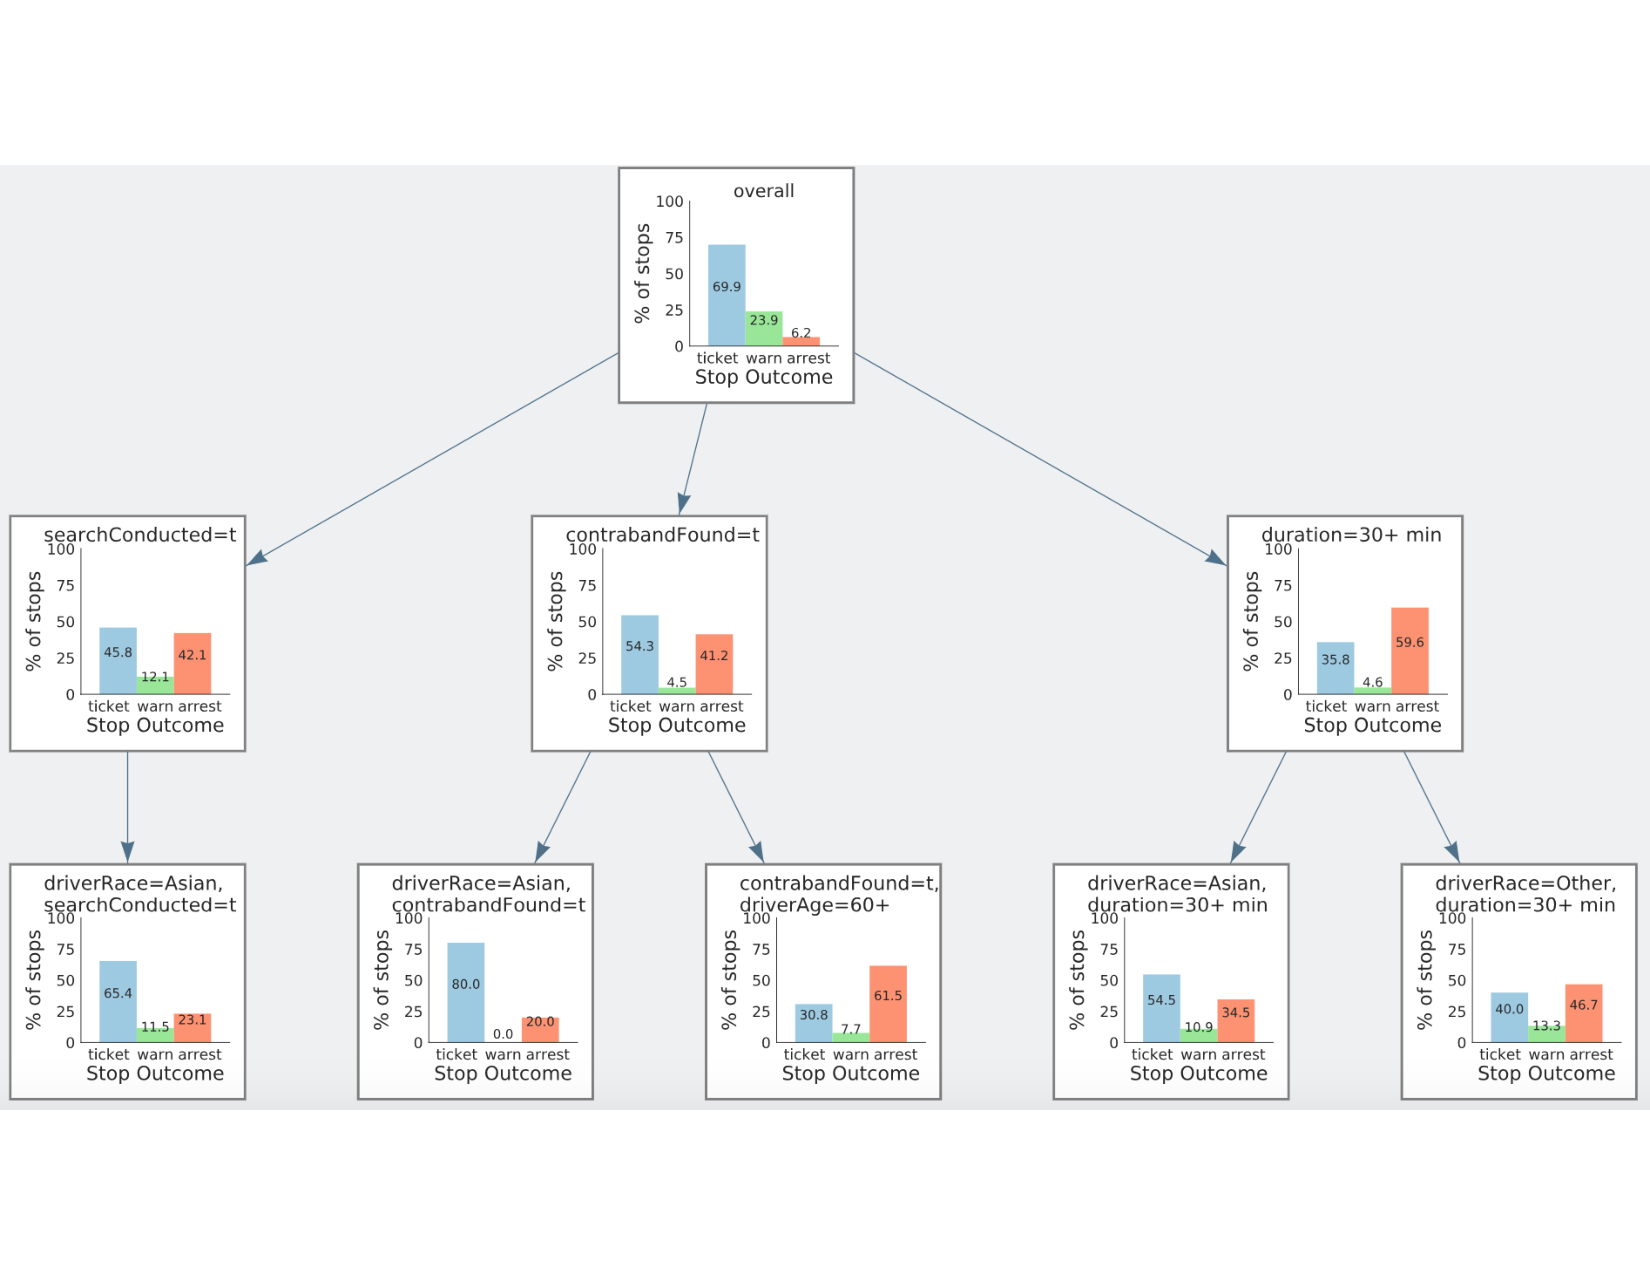
\includegraphics[width=0.7\linewidth]{figures/storyboard.pdf}
\caption{Example dashboard generated by \sbd summarizing the key insights in the Police dataset.}
\end{figure} 
% one paragraph on motivation on objectives and explain lattice + traversal 
\par While such summary dashboards are useful for making sense of relationships between data subsets, finding effective visualizations to summarize a dataset is not as trivial as picking individual visualizations that maximizes some statistical measure, such as deviation~\cite{Vartak2015}, coverage~\cite{Sarvghad2017}, or significance testing~\cite{Anand2015}, which can often result in misleading summarizations. The key insights of our work is understanding 

For example, our insight regarding 

The above example demonstrates a scenario where the selection of an improper reference (female) for comparing the visualization (black female) against results in misleading insights. In \sbd, we formulate an objective where a visualization is \emph{actually} interesting when it deviates from and can not be explained by \emph{even} its most informative reference.

%explain distribution awareness + its application, its relationship with dataset understnading + how it can be used in other contexts.
\par The effectiveness of \sbd largely comes from how it helps analysts become more \emph{distributionally aware} of the dataset. We define \emph{distribution awareness} as the aspect of data understanding in which analysts make sense of the key distributions across different data subsets and their relationship in the context of the dataset. So that even though it may be infeasible to examine all possible data subsets, with distribution awareness, the analyst will still be able to draw meaningful insights and establish correlations about related visualizations by generalizing their understanding to make predictions regarding the unseen visualizations. Our user study evaluations show that facillatating distribution awareness through \sbd guides users to make better predictions regarding unseen visualizations, ranking attribute importance, and retreival of interesting visualizations compared to the baselines.


%building future systems that effectively guide analysts towards more meaningful stories for further investigation.
% How ----- is underexplored 
% future research 
% building systems that ---

\subsection{Contextual and Situational Awareness: Challenges and Opportunities}
\par The notion of distribution awareness is useful when we are looking at user understanding at one static point in time of the analysis (e.g. during cold start). As a ---- future research, in this section, we introduce two complementary notions of data understanding (contextual and situational awareness) when considering dynamic visual exploration in the context of an analytic workflow.
 %In this section, we will discuss several other types of data understanding that is essential for effective visual data exploration. Recommendation providing better understanding for overall dataset and understanding. 
\stitle{Contextual awareness} is the aspect of data understanding that relates to understanding what is  current ------, including making sense of the data attributes and schema, keeping track of which filters or transformations have been applied to the displayed data.


serves to ---- in a dynamic exploration situation, keep track of what filter is in play, what dataset/ schema am I looking at, which operations have been applied to the data that I'm looking at? Related to provenance for the current time. 
Within a dataset, structure and provenance is essential to help users navigate and provide users with sense of coverage and completion. This is an important but underexplored area. (viz-sum, Sarvghad et al 2017)
\par Mechanisms that facillitate distribution awareness for users can effectively couple with contextual awareness in a dynamic exploration situations to help update the user's mental model on the current data context. For example, the representative and outlier patterns in \zv provides summaries of data in context. When a dataset is filtered, the representative trends are updated accordingly. By understanding both the context (i.e. I'm only looking at data filtered with ....), the users becomes distributionally aware of the data in the particular context. 
an overview of typical trends for the data to be queried.
% better understanding of what's in the dataset that I'm looking at. related also to interpretability 
\stitle{Situational awarenss}: 
related to provenance, as a function of time.
- provenance of schema and attribute understanding (coverage, etc) . Similar to situational awareness (cite Tory)

\par The key difference between contextual and situational awareness is that contextual awareness is focussed on how the current context of the data came about, whereas situational awareness accounts for all prior user actions to --- intent. For example, a user may be interested in how a measure variable changes when groupby upon different dimensions variables. The analyst may examine and clear various x-axis in sequence: contextual awareness informs the user that the context is the last attribute that has not yet been cleared, whereas situational awarness provides a notion of coverage informing the analyst that they have already explored this attribute.

\par Note that while the discussion above have been focussed on how to design systems that can help facillatate these aspects of user's awareness in dataset understanding, these ideas can be generalized to principles in deisinging the types of intelligent querying systems discussed in Section~\ref{sec:vague}. An intelligent visual exploration system needs to be distributionally, contextually and situationally aware, by make use of information about the data (distribution awareness), the analytic context, and situation jointly in making timely recommendations. For example, contextual awareness can inform the system that the user's current ---- x,y, main visualization, while a distributionally aware system may recommend a highly-skewed data subset as interesting, a sitational aware system may realize a variable have been explored extensively in the past and recommends it accordingly. In other words, these intelligent visual query system not only needs to facillatate these aspects of data understanding, but also need to make use of this information to make inference and recommendations in an interpretable manner that can guide analysts towards meaningful stories and insights for further investigation.

inference and descisions intepretable.

, rather than the system's awareness of the user's context, situation ,etc. Ideally, an intelligent system  should 


related works have focussed on making specification easier, but not really trying to understnad user intent or what might the user want to see.
